% ch05-shacl-mechanism.tex — SHACL Operational Flow
% Target → Focus Node → Path → Value Nodes → Constraint → Result
% Pedagogical purpose: make SHACL feel mechanistic, not just syntactic.
\documentclass[tikz,border=5pt]{standalone}
\usepackage{fontspec}
\setmainfont{Times New Roman}
\usepackage{unicode-math}
\setmathfont{Cambria Math}
\usetikzlibrary{shapes.geometric,shapes.misc,positioning,fit,backgrounds,arrows.meta}

\begin{document}
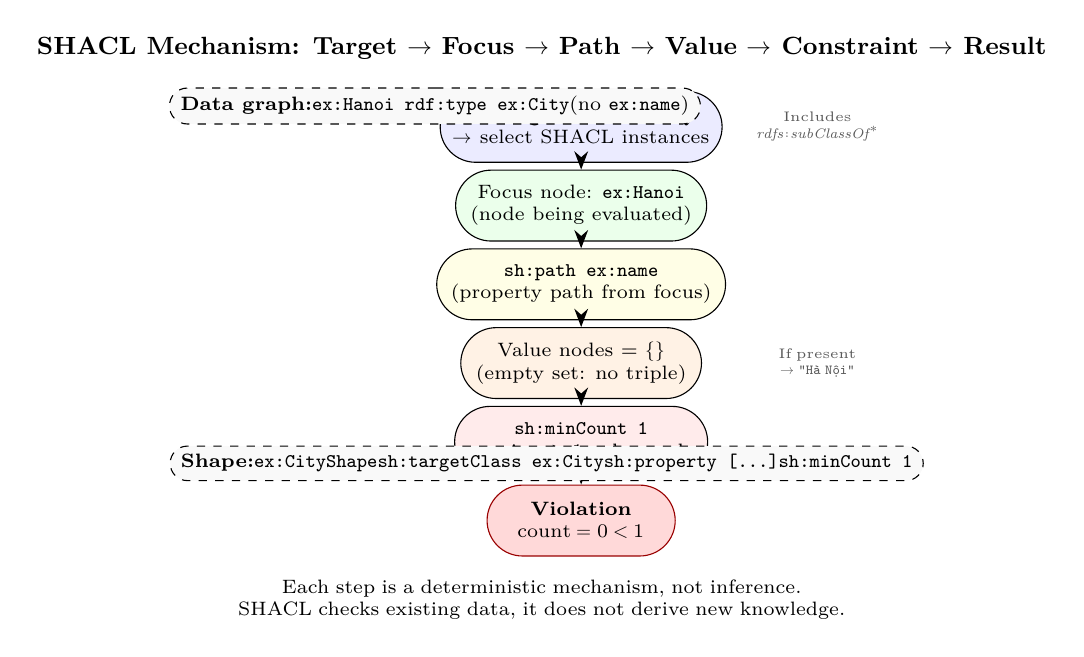
\begin{tikzpicture}[
  stepbox/.style={rounded rectangle,draw,minimum width=2.6cm,minimum height=0.9cm,
                  font=\scriptsize,align=center,inner sep=3pt},
  databox/.style={rounded rectangle,draw,dashed,font=\scriptsize,inner sep=3pt,
                  fill=gray!5,minimum width=2.4cm},
  arr/.style={->,>=Stealth,thick},
  steplabel/.style={font=\footnotesize\bfseries,text=blue!70!black,anchor=east},
  note/.style={font=\tiny,text=gray!70!black,align=center,text width=2.8cm},
]

% Title
\node[font=\small\bfseries] at (0,5.0) {SHACL Mechanism: Target $\to$ Focus $\to$ Path $\to$ Value $\to$ Constraint $\to$ Result};

% Step 1: Target
\node[steplabel] at (-1.8,4.0) {①};
\node[stepbox,fill=blue!8] (target) at (0.5,4.0) {\texttt{sh:targetClass ex:City}\\$\to$ select SHACL instances};
\node[note] at (3.5,4.0) {Includes\\$\mathit{rdfs\!:\!subClassOf}^*$};

% Step 2: Focus Node
\node[steplabel] at (-1.8,3.0) {②};
\node[stepbox,fill=green!8] (focus) at (0.5,3.0) {Focus node: \texttt{ex:Hanoi}\\(node being evaluated)};

% Step 3: Path
\node[steplabel] at (-1.8,2.0) {③};
\node[stepbox,fill=yellow!10] (path) at (0.5,2.0) {\texttt{sh:path ex:name}\\(property path from focus)};

% Step 4: Value Nodes
\node[steplabel] at (-1.8,1.0) {④};
\node[stepbox,fill=orange!10] (value) at (0.5,1.0) {Value nodes = $\{\}$\\(empty set: no triple)};
\node[note] at (3.5,1.0) {If present\\$\to$ \texttt{"Hà Nội"}};

% Step 5: Constraint
\node[steplabel] at (-1.8,0.0) {⑤};
\node[stepbox,fill=red!8] (constraint) at (0.5,0.0) {\texttt{sh:minCount 1}\\requires $\geq 1$ value node};

% Step 6: Result
\node[steplabel] at (-1.8,-1.0) {⑥};
\node[stepbox,fill=red!15,draw=red!60!black] (result) at (0.5,-1.0) {\textbf{Violation}\\$\mathrm{count}=0 < 1$};

% Arrows
\draw[arr] (target) -- (focus);
\draw[arr] (focus) -- (path);
\draw[arr] (path) -- (value);
\draw[arr] (value) -- (constraint);
\draw[arr] (constraint) -- (result);

% Data context box
\node[databox,anchor=north west] at (-4.5,4.5)
  {\textbf{Data graph:}\\
   \texttt{ex:Hanoi rdf:type ex:City}\\
   (no \texttt{ex:name})};

\node[databox,anchor=south west] at (-4.5,-0.5)
  {\textbf{Shape:}\\
   \texttt{ex:CityShape}\\
   \texttt{sh:targetClass ex:City}\\
   \texttt{sh:property [...]}\\
   \texttt{sh:minCount 1}};

% Bottom note
\node[font=\scriptsize,align=center,text width=8cm] at (0,-2.0)
  {Each step is a deterministic mechanism, not inference.\\
   SHACL checks existing data, it does not derive new knowledge.};

\end{tikzpicture}
\end{document}
